\section{Background determination}
\label{sec:background}

\subsection{Method of uncorrelated variables (ABCD)}
\label{subsec:abcd}
For background estimation we use a data driven method of independent selections, the "ABCD method", using
 three independent selection criteria listed in Section \ref{subsec:selection}. 
The three selection criteria divide the candidates into eight
independent regions as listed in Table \ref{tab:regions}.

\begin{table}[htbp]
\centering
\caption{Naming convention for the regions used in background estimation. "+" corresponds to a selection 
being applied, while "--" to a selection being inverted. \label{tab:regions}}
\begin{tabular}{cccc}
 \hline
  Region & selection 1 & selection 2 & selection 3 \\
 \hline
 A & -- & -- & -- \\
 B & + & -- & -- \\
 C & -- & + & -- \\
 D & -- & -- & + \\
 E & -- & + & + \\
 F & + & -- & + \\
 G & + & + & -- \\
 H & + & + & + \\
\hline
\end{tabular} 
\end{table}

The background level in the signal region H can be estimated from anyone of the 6 semi-independent combinations
of the candidate counts in other regions:
\begin{itemize}
\item FG/B, EG/C, EF/D - these combinations use 1 selection always applied, while applying and inverting the 
2 other selections;
\item DG/A, BE/A, CF/A - these combinations combine 2 selections together and apply or invert it with the 
remaining selection.
\end{itemize}

A seventh background prediction which minimizes statistical uncertainty, BCD/A$^2$, can be constructed from regions
with at least 2 selections inverted where background candidate counts are largest. 
We use BCD/A$^2$ as our background prediction central value. In the case of perfectly independent 
variables all combinations predict statistically consistent  amount of background. 
However, to account for possible systematic
effects due to residual dependence of the selections, we assign a systematic uncertainty as the maximal difference 
between BCD/A$^2$ and any of the 6 other predictions.

\subsection{Selection optimisation}
\label{subsec:cutvalues}
We determine the numerical values of the selection criteria that are employed in the background estimation procedure 
by optimizing expected limit for each tested signal model.
The signal models considered include various values of the \Higgs mass, the \X mass, and the \X lifetime.
The selection variables
do not strongly depend on the particles masses, therefore the optimal selection criteria
vary only as a function of the
mean transverse decay length ($L_{xy}$)
of the \X bosons. We use two sets of selection criteria,
depending on whether the mean
$L_{xy}$ of the \X bosons is below or above 30 \cm, respectively. The selection criteria are
detailed in Table \ref{tab:background}.

\begin{table}[htbp]
\centering
\begin{tabular}{r|c|c}
%\hline
$\bf L_{xy}$ &\bf  $\bf <20\cm (low)$ & \bf  $\bf >20\cm (high)$ \\
\hline
prompt tracks & $\leq1$ & $\leq1$ \\
%\hline
prompt energy fraction & $<0.15$ & $<0.09$ \\
%\hline
vertex/cluster disc. & $>0.9$ & $>0.8$  \\
\hline
\bf expected background & $\bf 1.60\pm0.26(stat.)\pm0.51(syst.)$ & $\bf 1.14\pm0.15(stat.)\pm0.52(syst.)$ \\
%\hline
\end{tabular}
\caption{Optimised selection criteria and the corresponding background expectations with their statistical and systematic uncertainties.\label{tab:background}}
\end{table}

\subsection{Background tests}
\label{subsec:backgroundtests}
The background estimation procedure described in Section \ref{subsec:abcd} is general and can be applied
to any dataset if the selections used are independent.
In this section we describe various closure tests performed in QCD Monte Carlo simulation and 
selected control regions in data. Plots shown in the following sections present the observed number
of candidates and all of the 7 combinations predicting the background level as described
 in Section \ref{subsec:abcd}.
Uncertainties are statistical only. For each of the tested selection points the background prediction 
and its uncertainty are obtained 
using the prescription from Section \ref{subsec:abcd}. The background prediction and its statistical 
and systematic uncertainties are
 not explicitly plotted given that all of the 7 combinations employed in its derivation are shown.  
The compatibility between predicted and observed background is estimated with a {\it p-value} for every measurement. 
%The {\it p-values} are then converted into {\it significances} using the normal distribution. 
 The {\it p-value}
is computed with respect to the estimated background probability density function (p.d.f.). 
The background prediction has an associated uncertainty, 
therefore the background p.d.f. is a Poissonian function convolved  
with a Gaussian error function. The probability of observing $n$ background events is given by:
\begin{equation}
B(n,b,\sigma_b)= \frac{1}{\sqrt{2\pi}\sigma_b} \int_{0}^{\infty} 
exp\left[ -\frac{\left(x-b\right)^2}{2\sigma_b^2}\right]\frac{x^n e^{-x}}{n!}dx
\label{eqn:bdensity}
\end{equation}
where $b$ is the background central value and $\sigma_b$ the total uncertainty.
The gaussian probability density of the background mean has been truncated at 
0 in order to avoid unphysical values. Such a truncation results in a not properly normalized p.d.f. in equation 
\ref{eqn:bdensity}, however the {\it p-values} computed according to equation \ref{eqn:pvalues} take the 
normalization into account.   
\begin{equation}
{\it p} (n_{obs},b,\sigma_b) = \sum_{k\geq n_{obs}} B(k,b,\sigma_b) / \sum_{k} B(k,b,\sigma_b)
\label{eqn:pvalues}
\end{equation}
The {\it p-values} are then converted into {\it significances} using the normal
 distribution. The {\it significances} are shown in the bottom plots (Figures 
\ref{fig:bkg_MC}-\ref{fig:10percent}) aligned to the corresponding background
measurements.  

\subsubsection{QCD Monte Carlo background prediction}
\label{subsubsec:bkgQCDMC}

Due to limited statistics of the QCD MC samples the displaced jet trigger requirement has been removed,
 only the HLT\_HT300 trigger selection is applied. Additionally, the background is estimated with looser
 selection on prompt tracks variables compared to the final selection. 
In order to validate the background prediction with 
the observed poissonian candidate counts the cross-section weights are removed, 
therefore this test serves only the purpose of identifying biases due to selections not being
perfectly independent, and cannot be translated
into background prediction in data.  
As shown in Figure \ref{fig:bkg_MC} good agreement between predicted and observed background level is found, 
and the discrepancy is not significant for the tested selection points. Therefore, we conclude that the  
bias due to variables being not perfectly independent is small in the QCD MC samples. 

\begin{figure}[htbp]
  \centering
  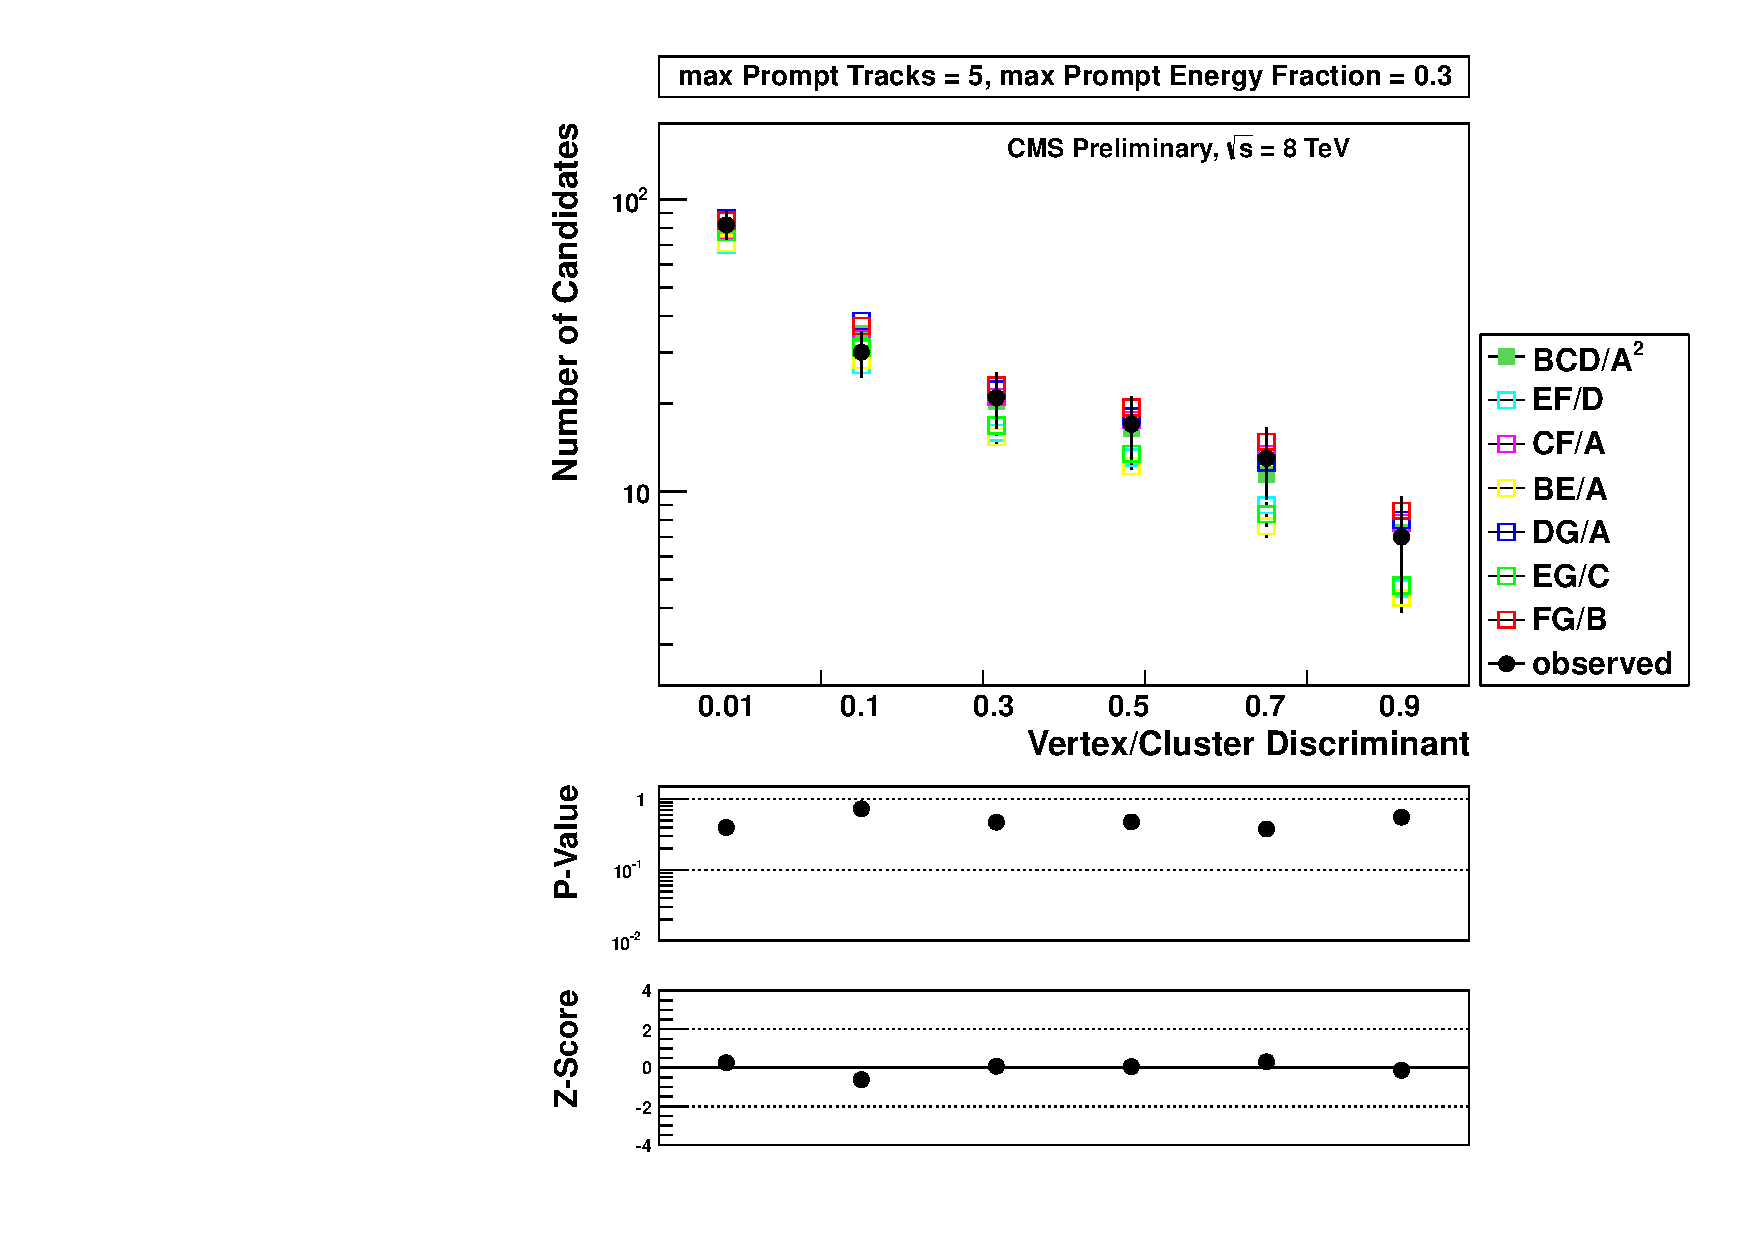
\includegraphics[width=0.495\textwidth]{plots/background/bkg_MC1.pdf}
  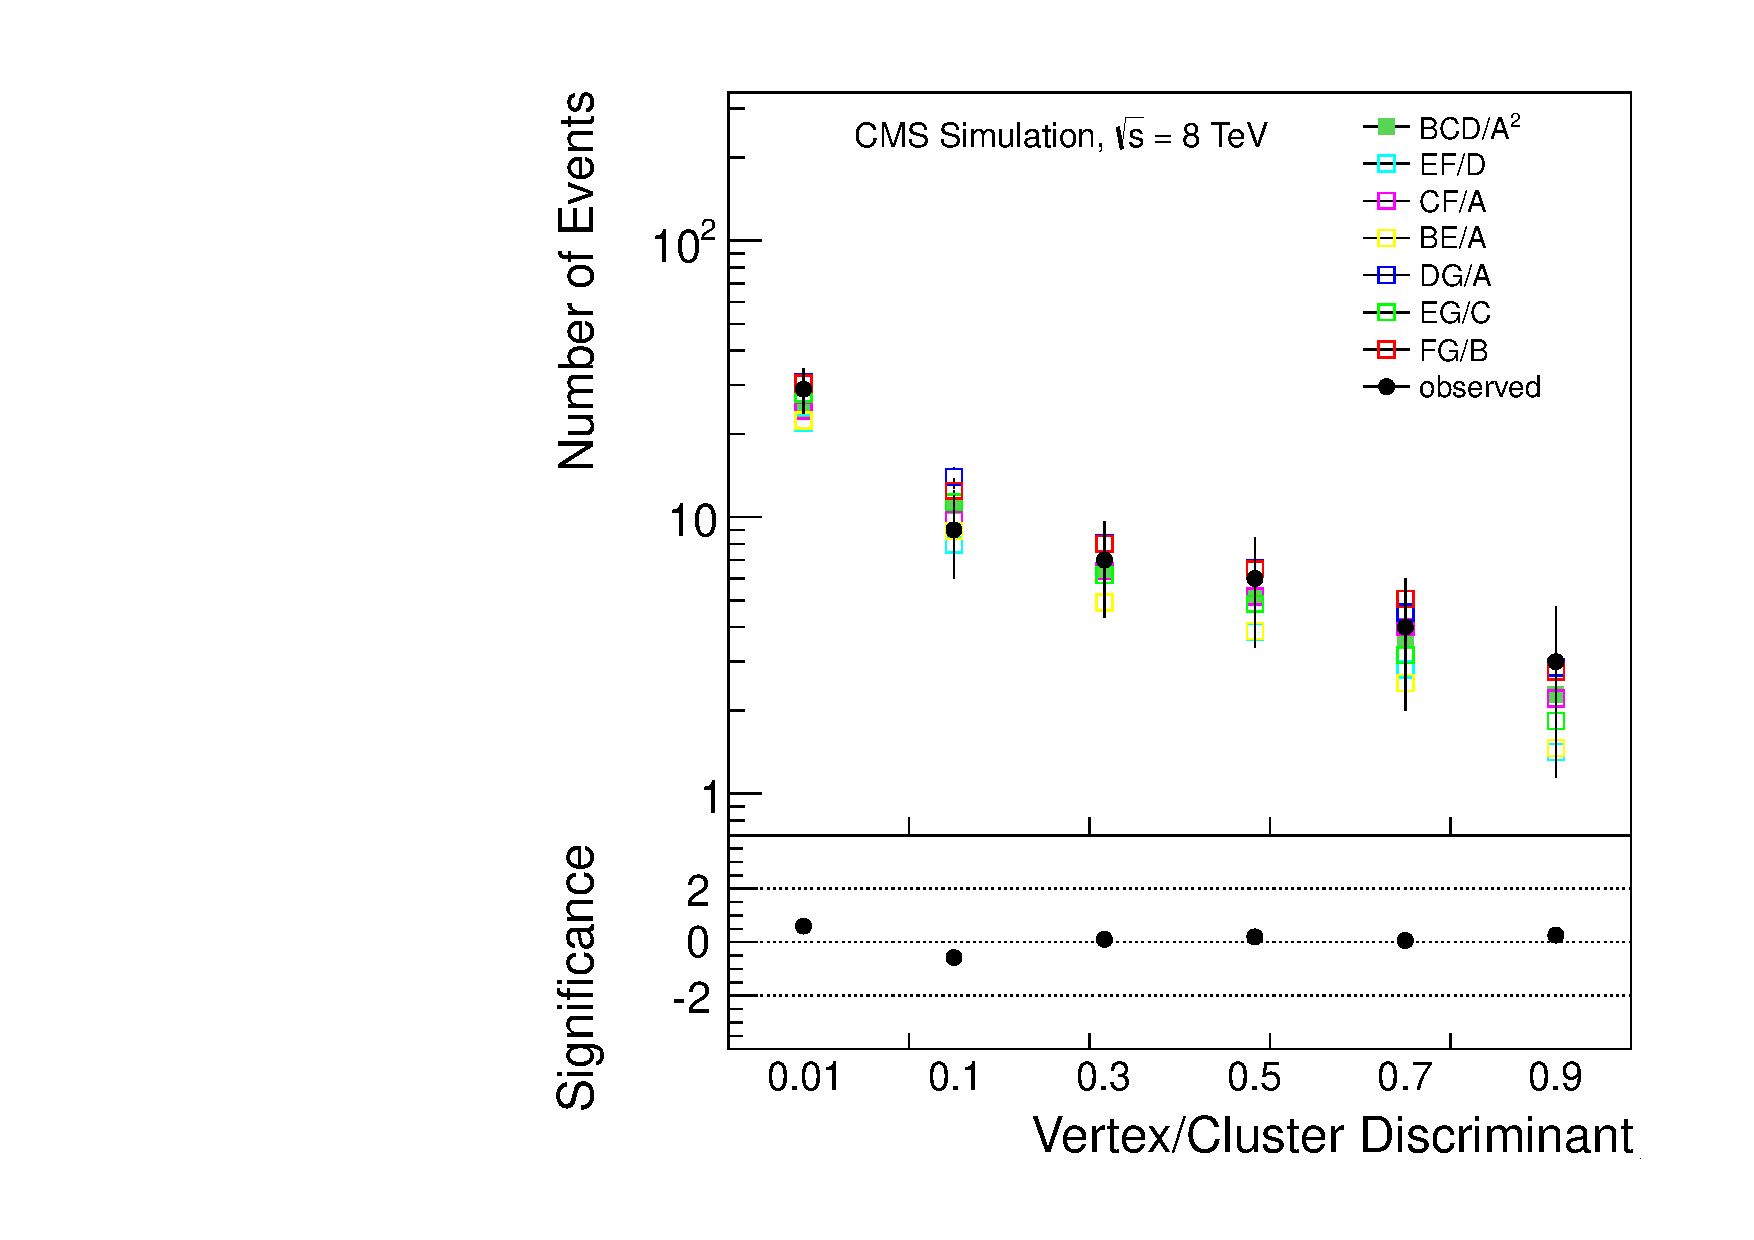
\includegraphics[width=0.495\textwidth]{plots/background/bkg_MC2.pdf}
  \caption{Predicted and observed background level for QCD Monte Carlo sample as a function of the vertex discriminant selection criteria.
Selection requires maximally 5 (left) and 4 (right)  prompt tracks and their jet energy fraction to be below 30\% (left) and 25\% (right) which
is significantly looser compared to final selection. \label{fig:bkg_MC}}
  \end{figure}


\subsubsection{Data control region}
\label{subsubsec:bkgCtrl}

As a data control region we use candidates passing all of the pre-selection criteria listed in Section
 \ref{subsec:selection} but with the {\it missing hits} selection inverted. Such a region has a very small 
signal acceptance compared to the signal region as the {\it missing hits} criterion has a very high signal 
efficiency, while providing
background sample with good statistics. Using this control region we are able to test final selection
criteria with amounts and uncertainties on predicted background comparable to the signal region. 
 As shown in Figure \ref{fig:bkg_NMiss}, 
the background predictions in this control region are in good agreement 
with the observed background level. Given that the significance
of the discrepancies is small, we conclude
that the background estimation method is valid and the systematic uncertainty on the background
 prediction is not underestimated.

\begin{figure}[htbp]
\centering
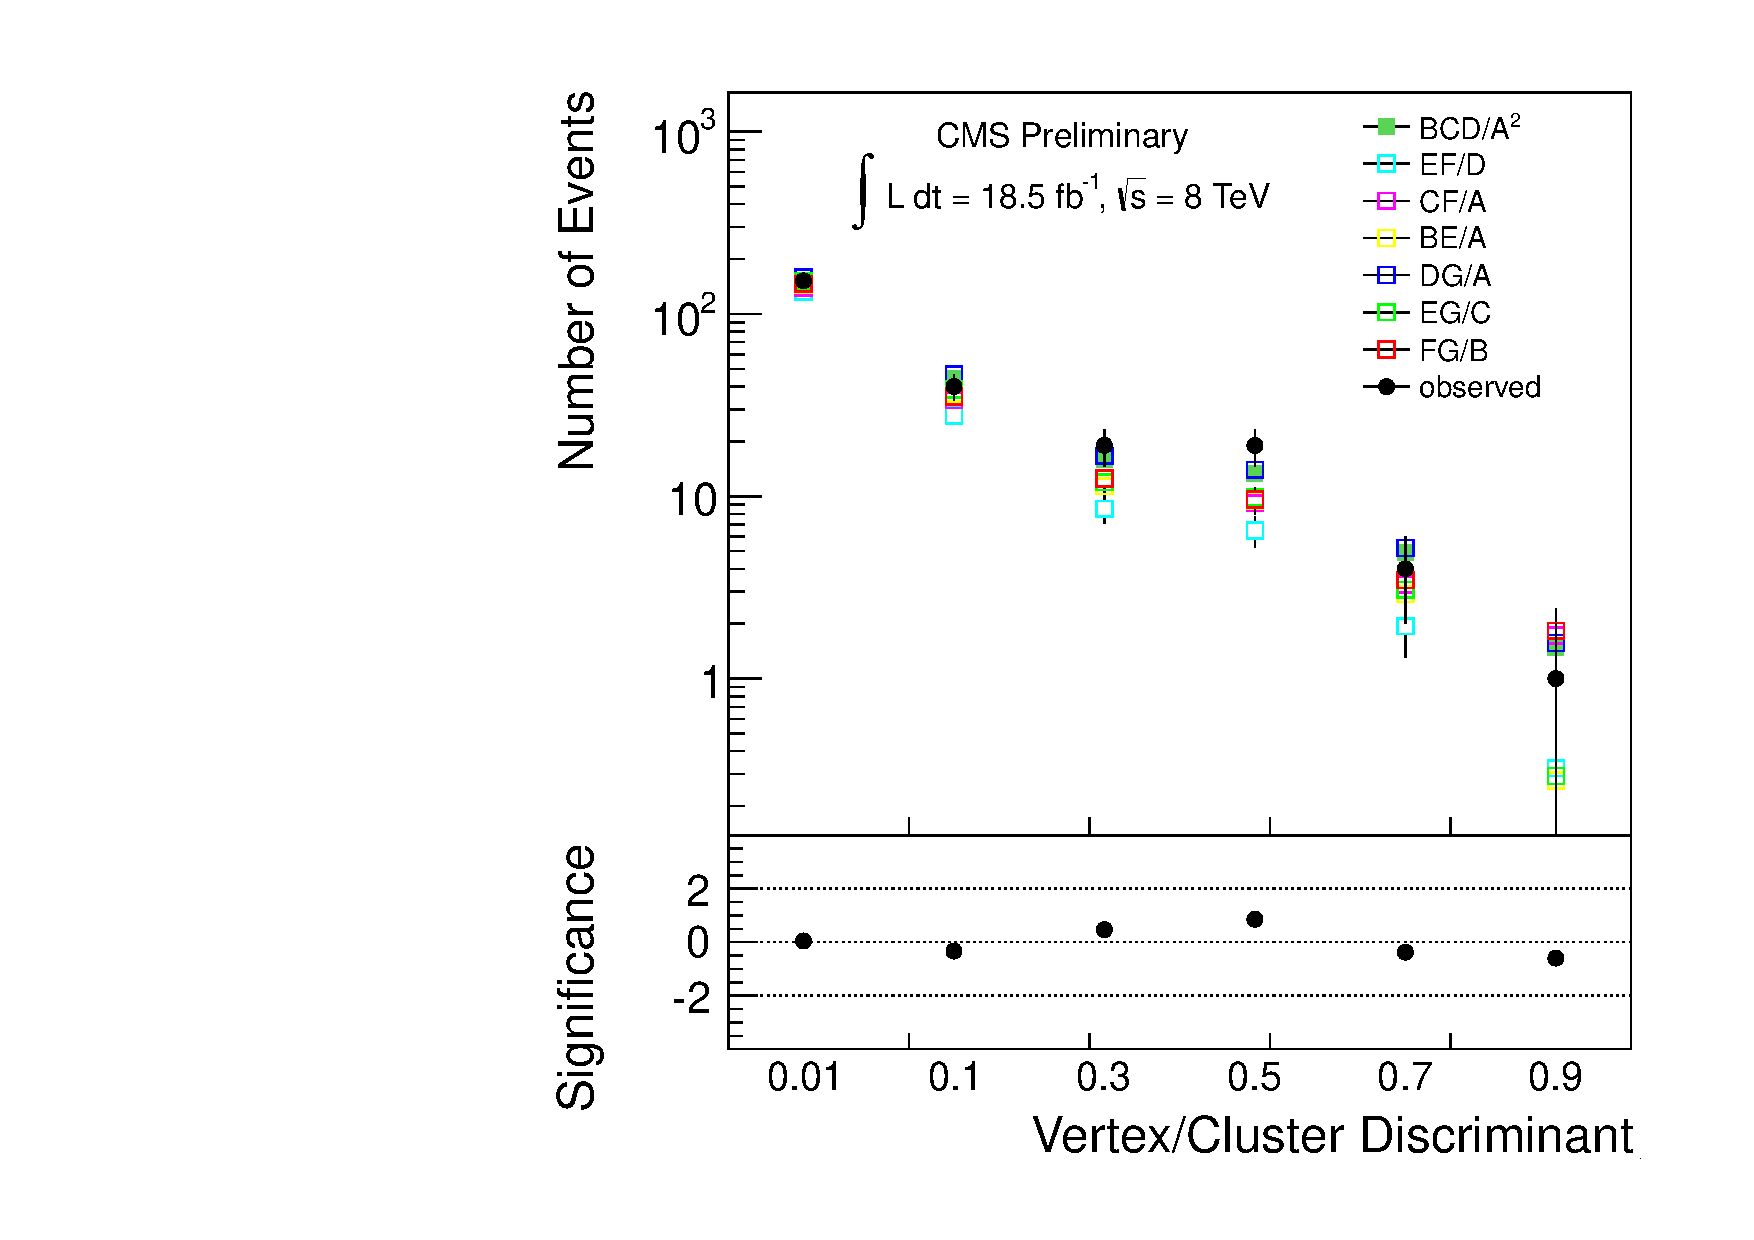
\includegraphics[width=0.495\textwidth]{plots/background/bkg_NMiss1.pdf}
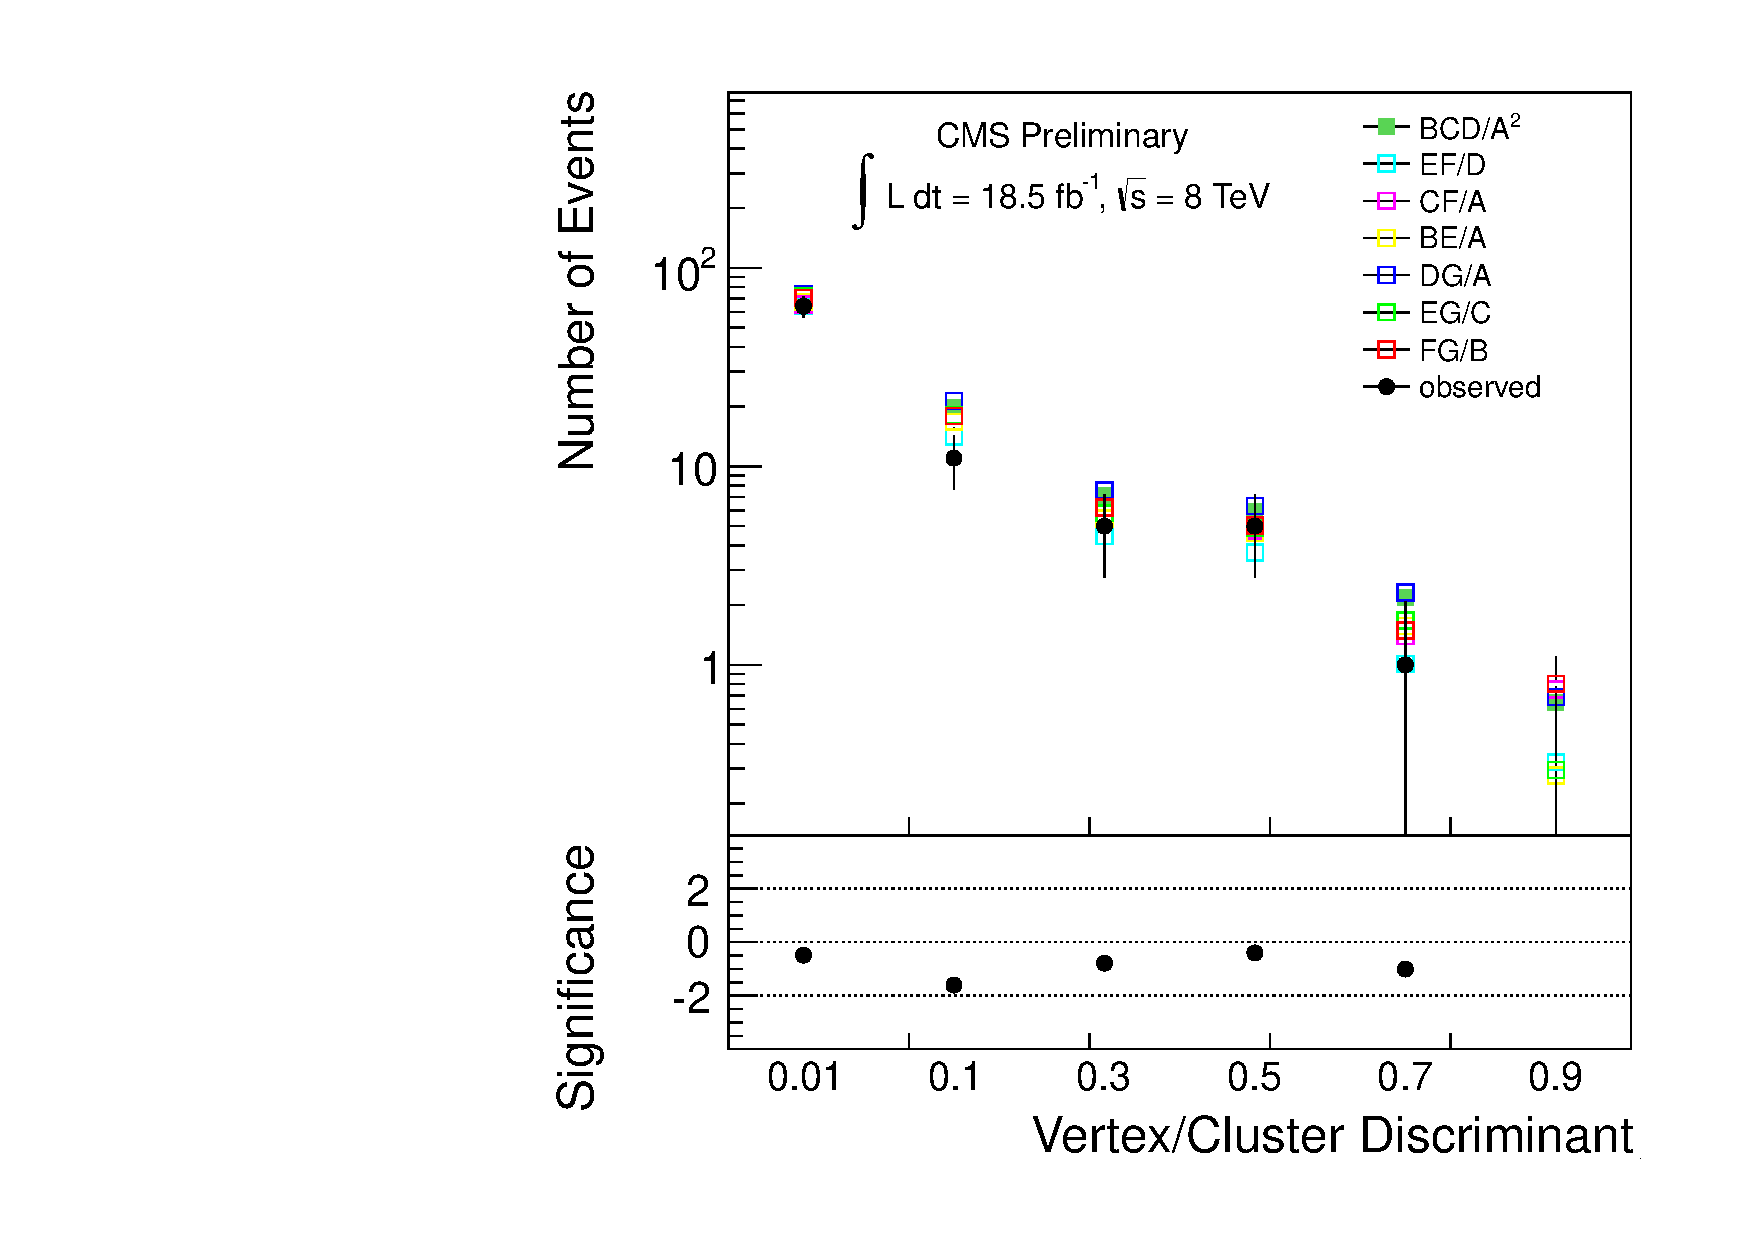
\includegraphics[width=0.495\textwidth]{plots/background/bkg_NMiss2.pdf}
\caption{Predicted and observed background level in the data control region as a function of the vertex
discriminant selection criteria. Selection requires maximally 1 prompt track and the prompt track energy fraction
is required to be less than 15\% and 9\% on the left and right plot respectively.\label{fig:bkg_NMiss}}
\end{figure}

\subsection{10\% unblinding}
\label{subsec:partunblinding}

In order to check that there is no anomalous background present,
 we initially examined the data corresponding to only 10\% of all available 
data in the signal region.  
We select the data using exactly 1 out of every 10 luminosity sections. This way of choosing 
the data is sensitive to possible issues that occur only for selected runs, and also for effects that may arise from
correlations between consecutive events accepted by the trigger. Comparison of the data and predicted
background is presented in Figure \ref{fig:10percent}. No anomalous background is observed in this sample,
however the background predictions are small therefore making the test statistically limited.

\begin{figure}[htbp]
  \centering
  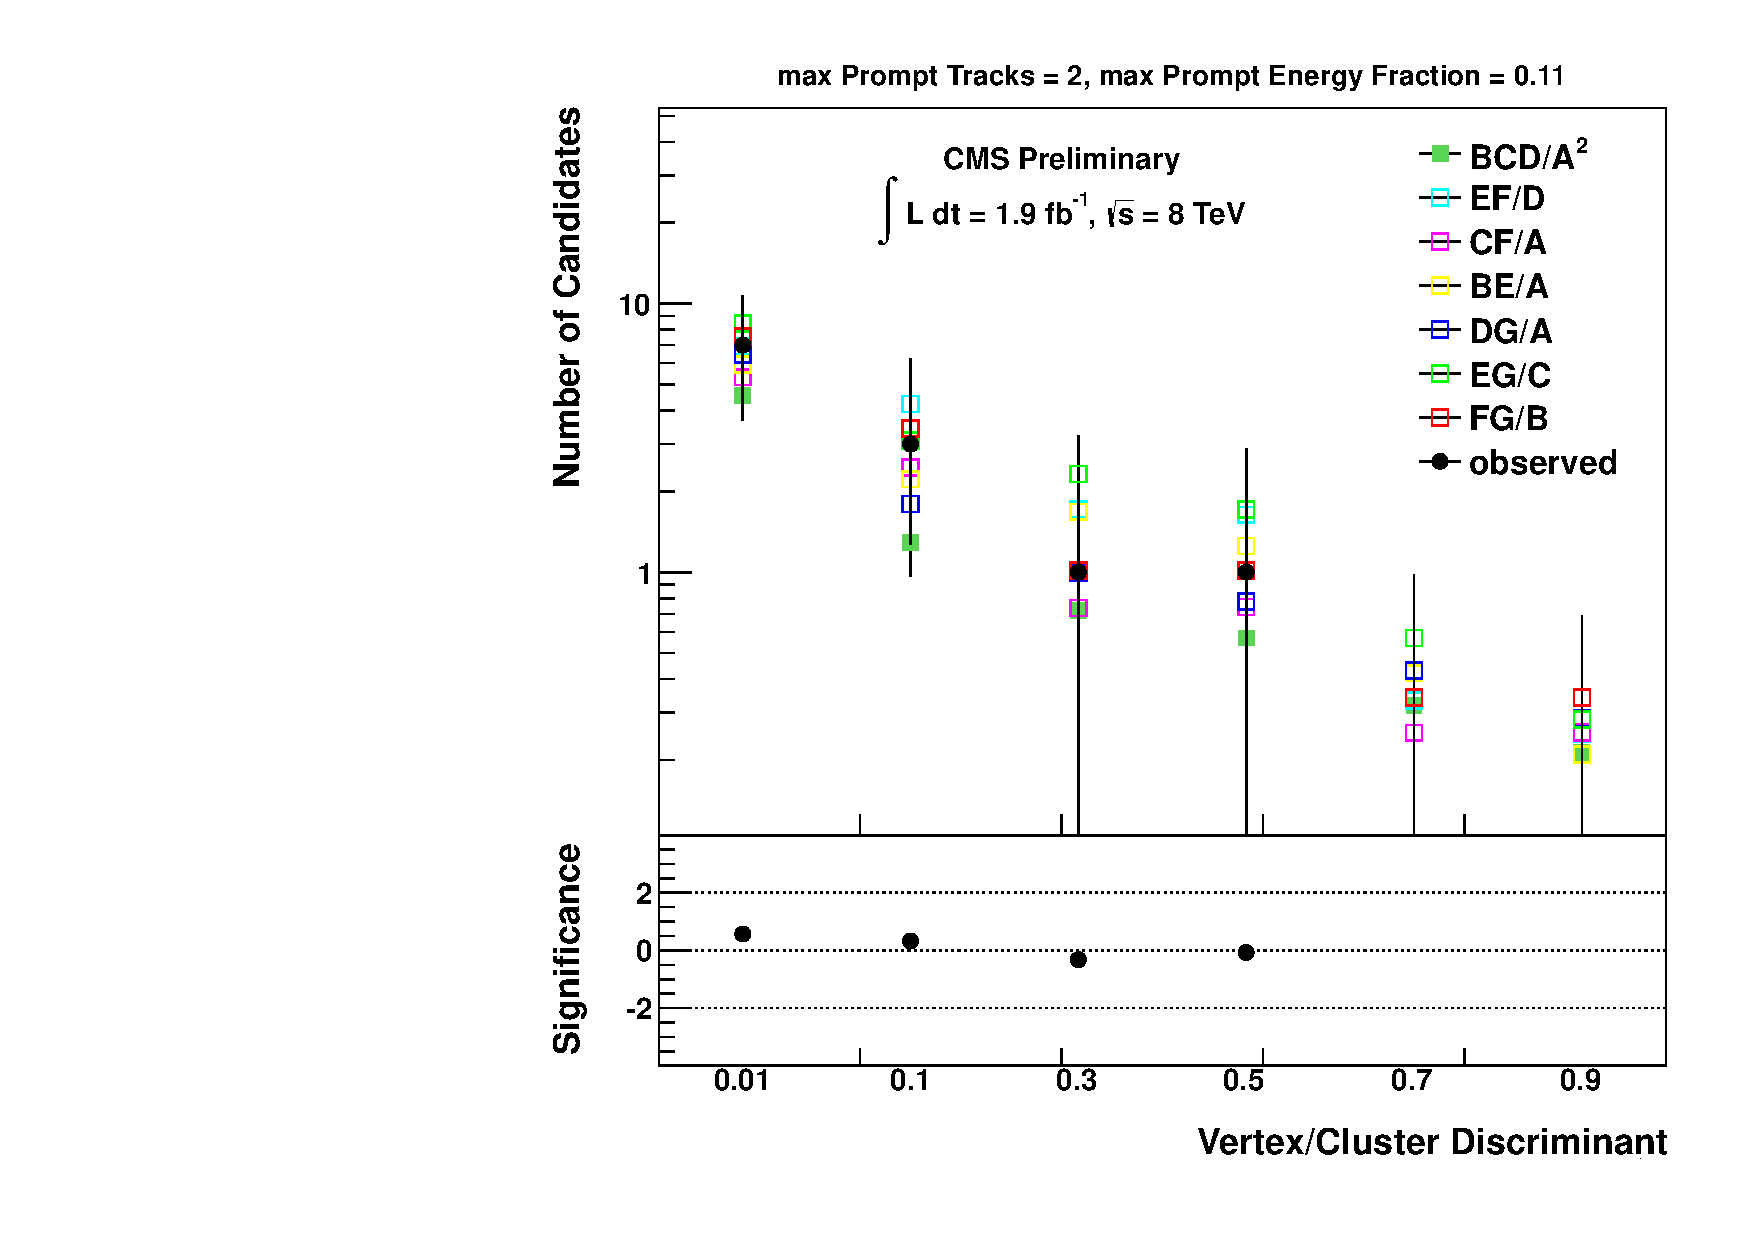
\includegraphics[width=0.495\textwidth]{plots/background/tenpercent1.pdf}
  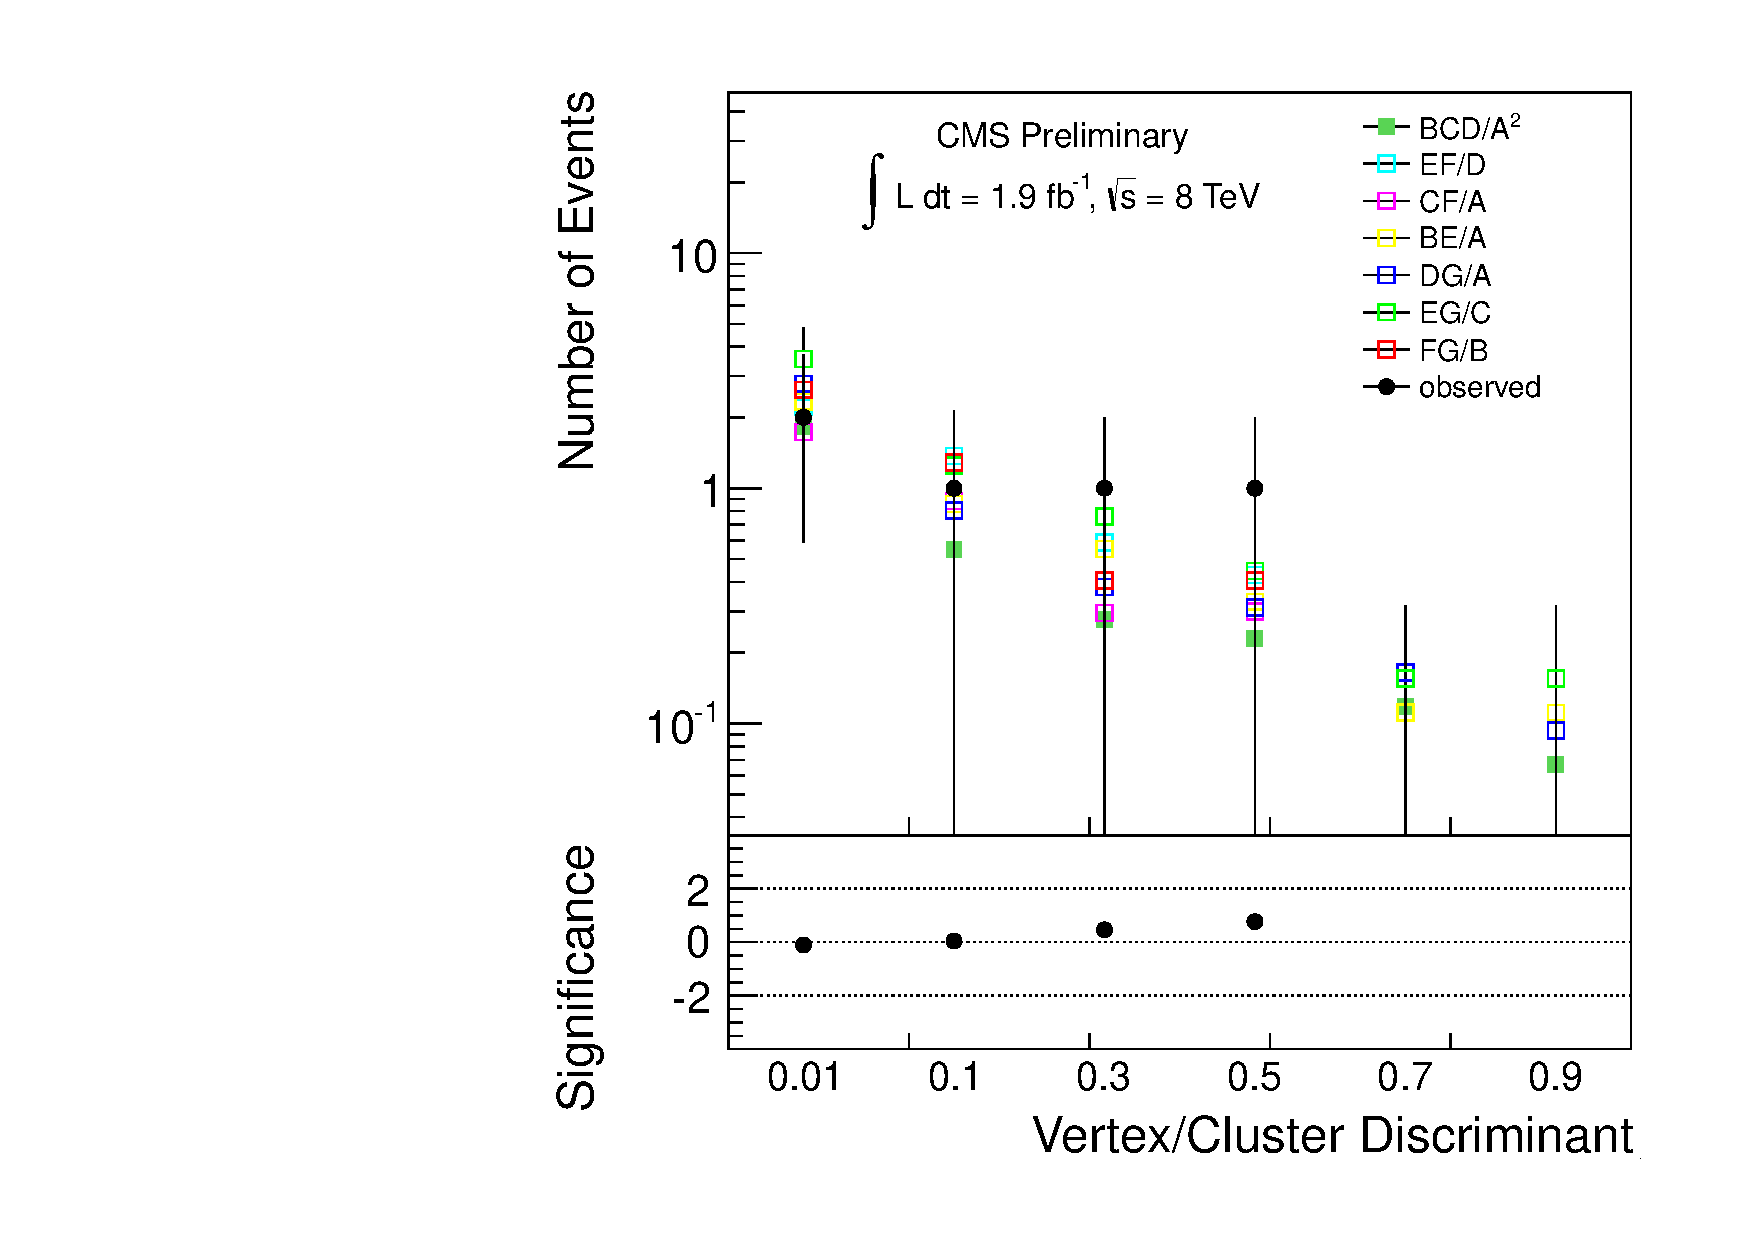
\includegraphics[width=0.495\textwidth]{plots/background/tenpercent2.pdf}
  \caption{Data and predicted background level in 10\% data sample as a function of vertex discriminant
selection criteria. Selection requires maximally 2 (left) or 1 (right) prompt tracks while the prompt track energy 
fraction is required to be less than 11\%. \label{fig:10percent}}
\end{figure}  


